\documentclass[12pt]{report}
\usepackage{graphicx}
\usepackage{color}

\begin{document}


\chapter{La Bioinformatique}

\begin{center}

\includegraphics[width=300]{bio.jpg} 
\end{center}






\newpage
\section{Intoduction}
La bioinformatique est une "interdiscipline" à la frontière de la biologie, de l'informatique et des mathématiques. Les systèmes biologiques sont très complexes et les techniques modernes d'investigation du monde biologique fournissent une vaste quantité de données expérimentales. Le but ultime de la bioinformatique est d'intégrer ces données d'origines très diverses pour modéliser les systèmes vivants afin de comprendre
et prédire leurs comportements (biologie systémique ou biologie des systèmes) dans des conditions de fonctionnement normales ou pathologiques. La bioinformatique est donc étroitement couplée à ses applications. Bon nombre de bioinformaticiens ne travaillent pas dans des laboratoires formellement estampillés \cite{ref18} . 
\\
Aujourd'hui , tout projet de biologie comporte une étape d'analyse bioinformatique des données. Par conséquent, un biologiste passe environ 20-30/100 de son temps à utiliser des outils bioinformatiques.\\
Ce chapitre décrit de manière simple les tâches courantes de la bioinformatique qu'un biologiste/biochimiste doit savoir traiter par lui-même, a partir les progrès de l'intelligence informatique pour la bioinformatique qui nous avons utiliser pour notre contexte d'étude qui représente l'application de l'apprentissage profond pour la prédiction de l'activité biologie \cite{ref18} .
\newpage
\section{Histoire du terme bioinformatique}
Le terme de bioinformatique date du début des années 80. Cependant, le concept sous-jacent de traitement de l'information biologique est bien plus vieux. Durant les années 60, la biologie moléculaire a eu besoin de modélisation formelle, ce qui a mené à la création des bioinformatique \cite{ref19}.\\
\section{Pour quoi la bioinformatique}
La bioinformatique est l'étude de l'information biologique. Ce n'est pas simplement l'application à la biologie de l'informatique, c'est une branche à part entière de la biologie. La bioinformatique actuelle se concentre surtout sur l'étude des séquences d'ADN et sur le repliement des protéines, donc travaille surtout au niveau moléculaire \cite{ref19} . 
\section{Qu'est-ce que la bioinformatique }
\subsection{Définition}
La bioinformatique est l'étude de l'information biologique de façon automatique, alors elle inclut la création et le développement de technologies informatiques qui permettant le traitement et l'analyse de ces information.
\\
l'intégration des méthodes mathématiques ,statistiques ,informatiques  pour analysées des données biologiques ,biochimiques et biophysiques \cite{ref20} .

\begin{figure}[h]

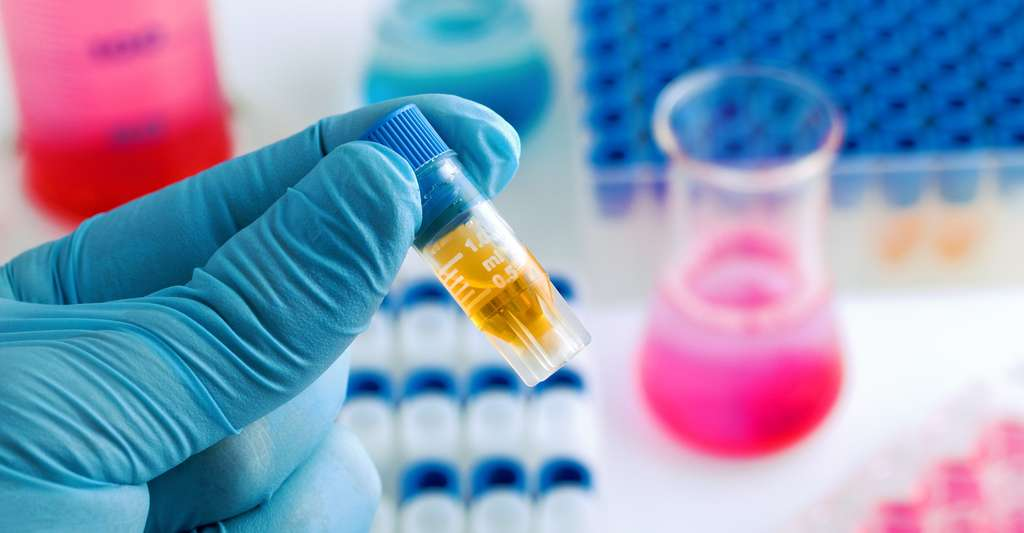
\includegraphics[width=200]{bb.jpg} 
\caption{premier image}
\label{premier image}

\end{figure}


La bioinformatique  se réfère spécifiquement à la recherche et à l'utilisation de  patterns et structures dans les données biologiques et au développement de nouvelles méthodes pour accéder aux bases de données \cite{ref20} .
\section{Apports à la biologie}
L'informatique est devenue un apport fondamentale à la biologie moléculaire. Les moyens informatiques sont naturellement utilisés pour le stockage ou la gestion des données mais également pour l'interprétation de ces données. Le traitement informatique des séquences peut par exemple déterminer la fonction biologique d'un gène. Cet apport informatique concerne principalement quatre aspects :
\begin{enumerate}
\item Le premier est l'organisation des données avec essentiellement la création de bases de données afin de réunir le plus d'information possible sur les séquences. 
\item Le deuxième aspect concerne les traitements que l'on peut effectuer sur les séquences afin de repérer un élément biologique intéressant. Ces programmes représentent les traitements couramment utilisés dans l'analyse des séquences comme la recherche des similitudes d'une séquence avec l'ensemble d'une base de données.
\item Le troisième aspect est celui qui permet d'élaborer des stratégies pour apporter des connaissances biologiques supplémentaires que l'on pourra ensuite intégrer dans des traitements standards. Par exemple la mise au point de nouvelles matrices de substitution des acides aminés,...etc
\item  Enfin, le quatrième aspect est celui de l'évaluation des différentes approches citées précédemment dans le but de valider.

\end{enumerate}





\section{Domaine d'application}
De plus en plus, la bioinformatique est développée dans un but d'application à l'agriculture, la pharmacologie, la  médecine \cite{ref21}. 
\newpage
\subsection{Structures moléculaires}
  Visualisation, analyse, classification, prédiction.
  \begin{figure}[h]
  \begin{center}
  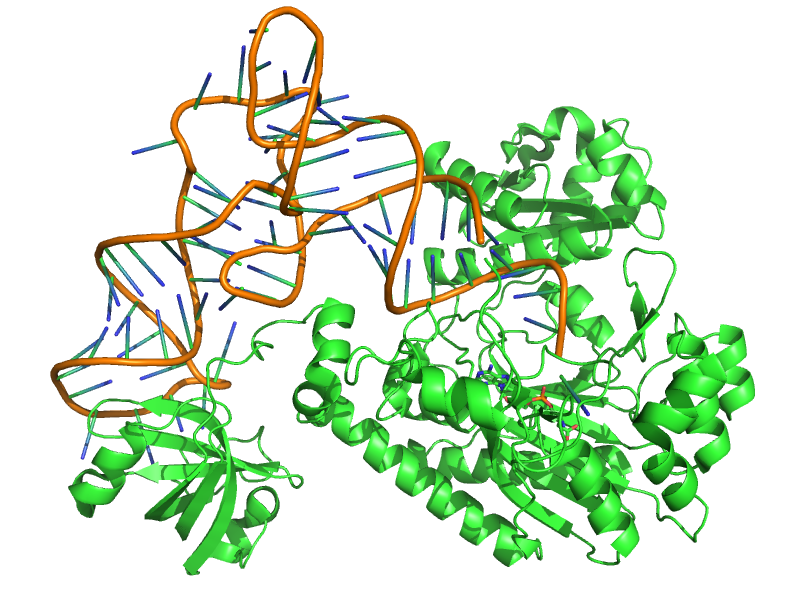
\includegraphics[width=200]{m.png} 
   \caption{La structure moléculaire}
  \end{center}  
  \end{figure}
  \subsection{Analyse de séquences}  
Alignements, recherches de similarités, détection de motifs.
\subsection{La recherche pharmaceutique}
\begin{enumerate}
\item Mécanismes d'action des médicaments.
\item Identification de cibles pharmaceutiques.
\end{enumerate}
\subsection{Génomique}
Annotation des génomes, génomique comparative.
\subsection{Analyse des réseaux biomoléculaires}
Réseaux métaboliques, d'interactions protéiques, de régulation génétique.

\newpage
\section{Quantitative et le système Pharmacologie (QSP)} 
La pharmacologie quantitative (QSP) est une nouvelle discipline sur l'identification et la validation de cibles de médicaments, comprendre les thérapeutiques existantes. Le but de QSP est de comprendre la manière précise et prédictive aussi comment les médicaments modulent les réseaux cellulaires dans l'espace et dans le temps et leur impact sur la physiopathologie humaine \cite{ref21}.\\
Au cours des trois dernières décennies, le paradigme dominant dans la découverte de médicaments a été la conception de ligands sélectifs pour une cible spécifique afin d'éviter les effets indésirables. Cependant, dans l'ère postgénomique actuelle, l'objectif est de concevoir des médicaments à partir les modèles de relations quantitatives structure-activité \textbf{QSAR} pour prédire la réponse biologique quantifiée d'une molécule à partir de ses descripteurs \cite{ref21} .

\section{Progrès de l'intelligence informatique pour la bioinformatique}
La bioinformatique est en train de devenir de plus en plus une science basée sur les données, une évolution tirée par les avancées technologiques en acquisition de données . Dans le domaine biomédical la grande quantité de données générées des scénarios difficiles pour les chercheurs, Les nouvelles exigences en matière de données requièrent de nouvelles approches en matière d'analyse des données. Certaines des plus intéressantes proviennent actuellement des domaines de l'intelligence computationnelle (IC) et de l'apprentissage automatique (ML) \cite{ref21}.\\
Cette session s'intéresse particulièrement à la proposition d'approches  de l'apprentissage automatique ML pour résoudre les problèmes dans les domaines biomédical et bioinformatique. Les sujets qui intéressent cette session :
\begin{enumerate}

\item \textbf{ Application de l'apprentissage profond pour la prédiction de l'activité biologique.}
\item Nouvelles applications des méthodes existantes d'apprentissage automatique ML à la bioinformatique.
\item Nouvelles techniques de d'apprentissage automatique ML pour la biomédecine et la bioinformatique.

\end{enumerate}
\newpage
\section{l'apprentissage profond et la modélisation Qsar}
\subsection{QSAR}
Relations entre l'industrie pharmaceutique et les modèles de relations quantitatives structure-activité (QSAR) pour prédire la réponse biologique quantifiée d'une molécule à partir de ses descripteurs, qui sont essentiellement des études étudiées de la molécule.

\begin{figure}[h]
\begin{center}
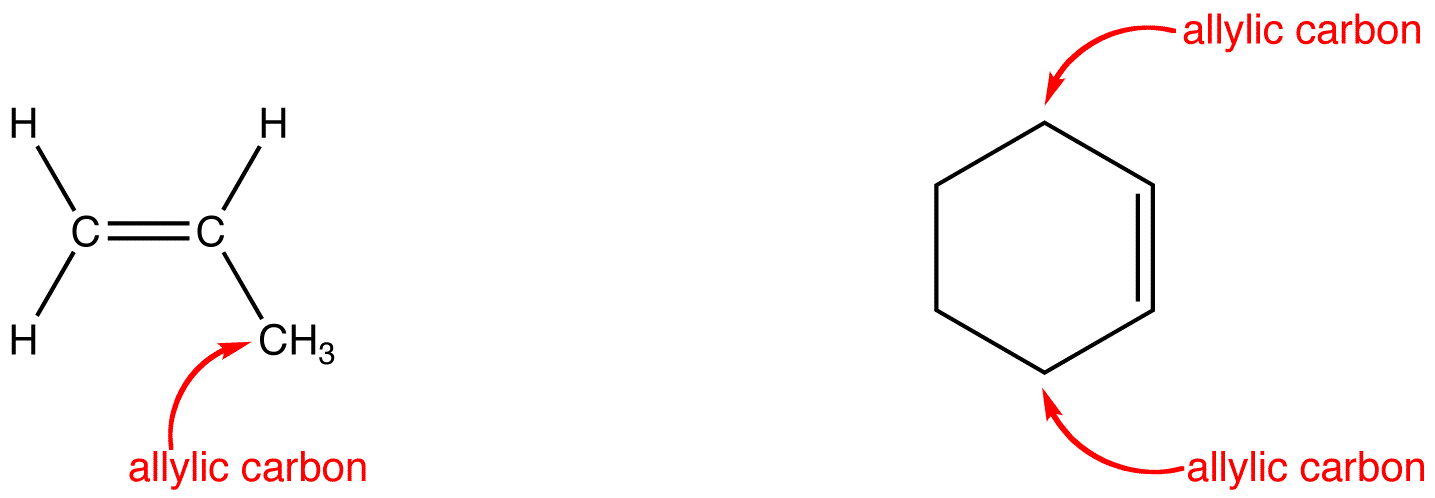
\includegraphics[width=250]{qsar.png} 
\caption{Allylic carbon}
\label{Allylic carbon}
\end{center}
\end{figure}
 
La complexité de ces descripteurs varie et peut aller de simples mesures de poids moléculaire à des caractéristiques géométriques complexes. La découverte de médicaments est un processus long et coûteux pour le secteur pharmaceutique.
\subsection{L'apprentissage en profondeur}
L'apprentissage en profondeur (deep learning) est un ensemble de méthodes d'apprentissage automatique et Les algorithmes d'apprentissage automatique, permettent aux ordinateurs de s'entrainer sur les entrées de données et utilisent l'analyse statistique .\\
fondées sur l'apprentissage de modèles de données, Une observation (une image, p. ex.) peut être représentée de différentes façons par un vecteur de données. Certaines représentations et une bonne capacité d'analyse automatique des différenciations rendent la tache d'apprentissage plus efficace \cite{ref22}.

\newpage
\subsection{La prédiction de l'activité biologique}
Le principe de la modélisation \textbf{Qsar}, consiste à trouver une relation reliant quantitativement une \textbf{activité biologique} mesurée expérimentalement. Ceci, est réalisé pour une série de composes similaire avec des descripteurs moléculaires à l'aide des méthodes computationnelles.\\
Les données des molécules biologiques disponibles dans les benchmarks sont tellement volumineuses (Big Data), qu'ils en deviennent difficiles à l'analyser avec des techniques de traitement de données classiques. Afin d'arriver à analyser ce type de données,nous faisant appel à des algorithmes de \textbf{Deep Learning }, qui sont en constante augmentation dans plusieurs domaines \cite{ref22}.

\section{Utilisation de l'amarrage (Docking)}
Dans le domaine de la modélisation moléculaire, l'amarrage est une méthode qui calcule l'orientation préférée d'une molécule vers une seconde lorsqu'elles sont liées pour former un complexe stable. Savoir l'orientation préférée sert à prévoir la solidité de l'union entre deux molécules \cite{ref23} .
\begin{figure}[h]
\begin{center}
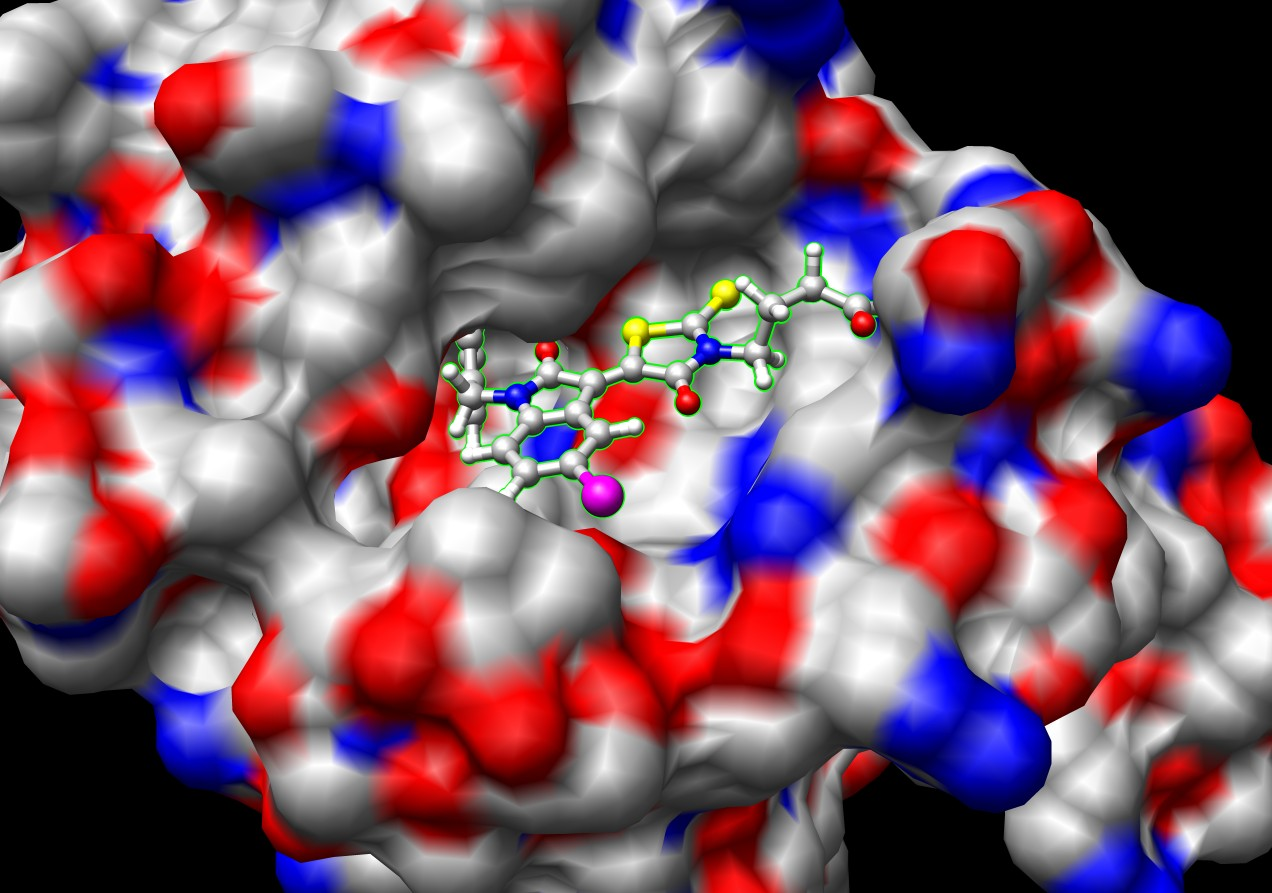
\includegraphics[width=200]{Docking.jpg}
\end{center}
\caption{Docking}
\end{figure}

 Les associations entre des molécules d'importance biologique, telles que les protéines, les acides nucléiques, les glucides et matières grasses jouent un rôle essentiel dans la transduction de signal. D'ailleurs, l'orientation relative des deux molécules associées peuvent avoir un effet sur le genre du signal produit (ex. antagoniste contre l'agoniste ). Par conséquent, des études d'amarrage sont utiles à calculer la force et le genre du signal produit  \cite{ref23} .\\
 Dans la mise au point de nouveaux médicaments, l'amarrage sert souvent à déterminer l'orientation de petites molécules liées à leurs protéines ciblées afin de calculer leurs affinité et niveau d'activité.



\section{Conclusion}
Dans ce chapitre nous avons définit les notions et l'évolution de la \textbf{bioinformatique} d'après le concept traitement de l'information biologique. les caractéristiques aussi les domaine d'application de la bioinformatique ,vers le problème biologique a traité sous domaine de la pharmacologie, d'objectif la prédiction de l'activité biologique pour concevoir des médicament à partir le modèle quantitative QSAR avec les moyennes informatique qui représente technique de l'apprentissage automatique (ML) qui fais appel à des algorithmes de Deep learning.\\
Dans le prochain chapitre nous allons exprimé notre démarche d'étude, aussi les outils de développement  utilisés tel que  le langage de programmation, sous chapitre de contribution.

\newpage
\bibliographystyle{plain}
\bibliography{biblio}

\end{document}
